\documentclass{article}

\usepackage{amsmath,amssymb,amsthm,graphicx,subfigure}

\pagestyle{myheadings}

\pdfpagewidth 8.5in
\pdfpageheight 11 in

\setlength\topmargin{0in}
\setlength\textheight{8.5in}
\setlength\textwidth{6.5in}
\setlength\oddsidemargin{0in}
\setlength\evensidemargin{0in}

\newcommand{\suchthat}{\ni}
\newcommand{\onlyif}{\Longleftrighttriangle}
\newcommand{\definedby}{\triangleq}
\newcommand{\union}{\bigcup}
\newcommand{\intersect}{\bigcap}
\newcommand{\where}{\mid}
\newcommand{\inverse}{\overline}

\title{CIT 596 Homework 1}
\author{Steven Tomcavage\\stomcava@seas.upenn.edu}
\date{February 3, 2011}

\markboth{\hfill Steven Tomcavage }{\hfill Steven Tomcavage }

\begin{document}

\maketitle

\section{Exercise 1.4}

\subsection{Exercise 1.4 e}

Create a DFA that accepts the language $\{ \omega \where \omega \text{ starts
with an } a \text{ and has at most one } b \}$.

\begin{figure}[h!]
	\centering
	\subfigure[$A$ accepts $\{\omega \where \omega \text{ starts with an } a \}$] 
	{
		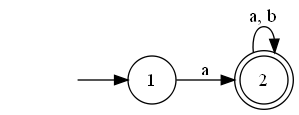
\includegraphics[height=1.0in]{1_4_e_a.png}
	}
	\subfigure[$B$ accepts $\{\omega \where \omega \text{ has at most one } b \}$] 
	{
		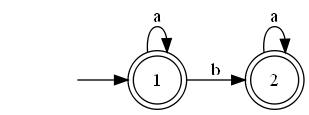
\includegraphics[height=1.0in]{1_4_e_b.png}
	}
	\subfigure[DFA that accepts $AB$] 
	{
		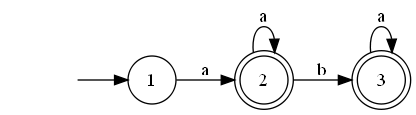
\includegraphics[height=1.0in]{1_4_e.png}
	}
	\caption{DFA for Exercise 1.4e}
\end{figure}

\newpage

\subsection{Exercise 1.4 f}

Create a DFA that accepts the language $\{ \omega \where \omega \text{ has
an odd number of } a \text{'s and ends with a } b \}$.

\begin{figure}[h!]
	\centering
	\subfigure[$A$ accepts $\{\omega \where \omega \text{ has an odd number of }
	a \text{'s}\}$] {
		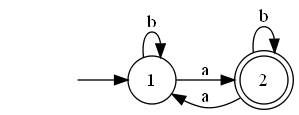
\includegraphics[height=1.0in]{1_4_f_a.png}
	}
	\subfigure[$B$ accepts $\{\omega \where \omega \text{ ends with a } b \}$] 
	{
		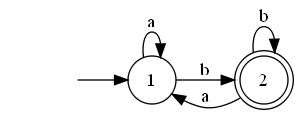
\includegraphics[height=1.0in]{1_4_f_b.png}
	}
	\subfigure[DFA that accepts $AB$] 
	{
		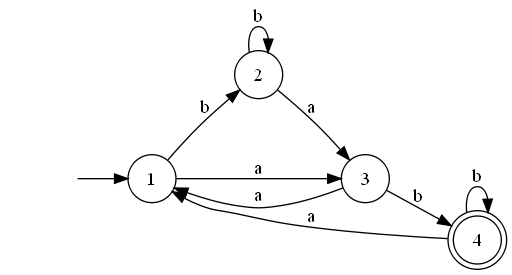
\includegraphics[height=2.0in]{1_4_f.png}
	}
	\caption{DFA for Exercise 1.4f}
\end{figure}

\subsection{Exercise 1.4 g}

Create a DFA that accepts the language $\{\omega \where \omega \text{ has
an even length and an odd number of } a \text{'s}\}$.

\begin{figure}[h!]
	\centering
	\subfigure[$A$ accepts $\{\omega \where \omega \text{ has an even length}\}$] {
		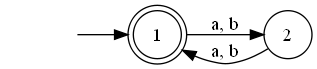
\includegraphics[height=0.75in]{1_4_g_a.png}
	}
	\subfigure[$B$ accepts $\{\omega \where \omega \text{ has an odd number of }
	a \text{'s}\}$] {
		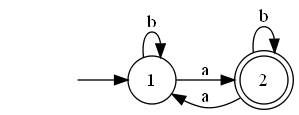
\includegraphics[height=1.0in]{1_4_g_b.png}
	}
	\subfigure[DFA that accepts $AB$] 
	{
		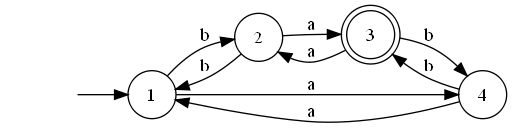
\includegraphics[height=1.0in]{1_4_g.png}
	}
	\caption{DFA for Exercise 1.4g}
\end{figure}

\section{Exercise 1.5}

\subsection{Exercise 1.5 c}

Create a DFA that accepts the language $\{ \omega \where \omega \text{
conains neither the substrings } ab \text{ nor } ba \}$.

\begin{figure}[h!]
	\centering
	\subfigure[$A$ accepts $\{\omega \where \omega \text{ contains } ab \text{ and
	} ba \}$] {
		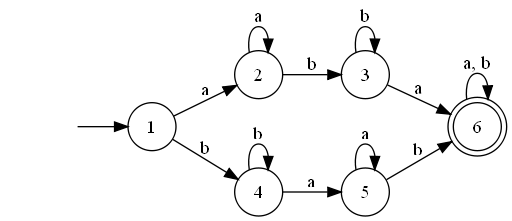
\includegraphics[height=2.0in]{1_5_c_a.png}
	}
	\subfigure[DFA that accepts $\inverse{A}$] 
	{
		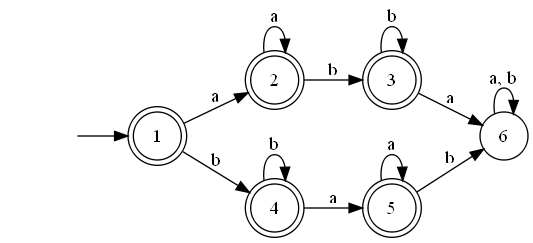
\includegraphics[height=2.0in]{1_5_c.png}
	}
	\caption{DFA for Exercise 1.5c}
\end{figure}

\newpage

\subsection{Exercise 1.5 e}

Create a DFA that accepts the language $\{ \omega \where \omega \text{ is
any string not in } (ab^\star)^\star \}$.

\begin{figure}[h!]
	\centering
	\subfigure[$A$ accepts $\{\omega \where \omega \text{ is in } (ab^\star)^\star
	\}$] {
		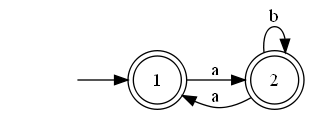
\includegraphics[height=1.0in]{1_5_e_a.png}
	}
	\subfigure[DFA that accepts $\inverse{A}$] 
	{
		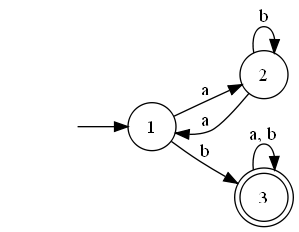
\includegraphics[height=2.0in]{1_5_e.png}
	}
	\caption{DFA for Exercise 1.5e}
\end{figure}

\subsection{Exercise 1.5 f}

Create a DFA that accepts the language $\{ \omega \where \omega \text{ is
any string not in } a^\star \union b^\star \}$.

\begin{figure}[h!]
	\centering
	\subfigure[$A$ accepts $\{\omega \where \omega \text{ is in } a^\star \union
	b^\star \}$] {
		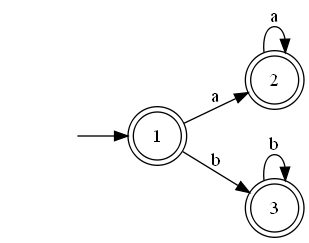
\includegraphics[height=2.0in]{1_5_f_a.png}
	}
	\subfigure[DFA that accepts $\inverse{A}$] 
	{
		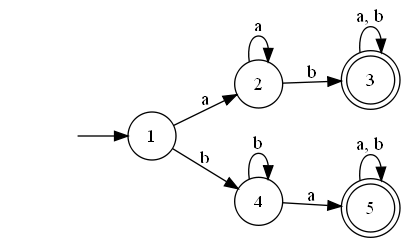
\includegraphics[height=2.0in]{1_5_f.png}
	}
	\caption{DFA for Exercise 1.5f}
\end{figure}

\newpage

\section{Exercise 1.6}

\subsection{Exercise 1.6 c}

Create a DFA that accepts the language $\{ \omega \where \omega \text{ contains
} 0101 \}$.

\begin{figure}[h!]
	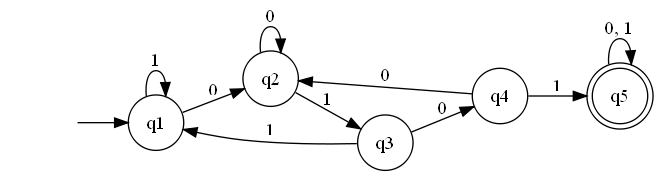
\includegraphics[height=1.5in]{1_6_c.png}
	\caption{DFA for Exercise 1.6c}
\end{figure}

\subsection{Exercise 1.6 e}

Create a DFA that accepts the language $\{ \omega \where \omega $ starts
with $0$ and has an odd length or $\omega$ starts with $1$ and has an even
length$\}$.

\begin{figure}[h!]
	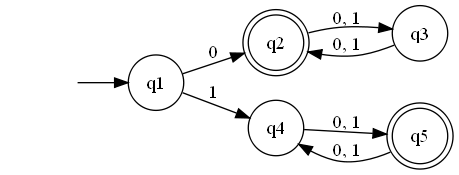
\includegraphics[height=1.5in]{1_6_e.png}
	\caption{DFA for Exercise 1.6e}
\end{figure}

\subsection{Exercise 1.6 g}

Create a DFA that accepts the language $\{ \omega \where \text{the length of }
\omega \text{ is at least } 5 \}$.

\begin{figure}[h!]
	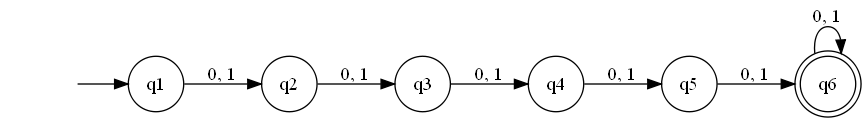
\includegraphics[height=0.75in]{1_6_g.png}
	\caption{DFA for Exercise 1.6g}
\end{figure}

\newpage

\subsection{Exercise 1.6 i}

Create a DFA that accepts the language $\{ \omega \where \text{every odd
position of } \omega \text{ is a } 1 \}$.

\begin{figure}[h!]
	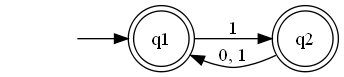
\includegraphics[height=0.75in]{1_6_i.png}
	\caption{DFA for Exercise 1.6i}
\end{figure}

\subsection{Exercise 1.6 j}

Create a DFA that accepts the language $\{ \omega \where \text{contains at
least two 0s and at most one 1} \}$.

\begin{figure}[h!]
	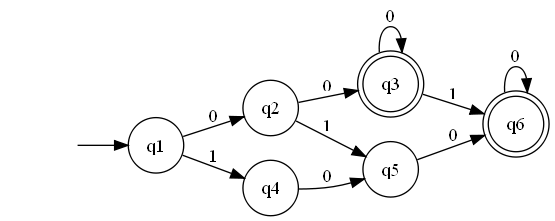
\includegraphics[height=2.0in]{1_6_j.png}
	\caption{DFA for Exercise 1.6j}
\end{figure}

\section{}

TODO

\section{}

TODO

\end{document}
